%Copyright 2014 Jean-Philippe Eisenbarth
%This program is free software: you can 
%redistribute it and/or modify it under the terms of the GNU General Public 
%License as published by the Free Software Foundation, either version 3 of the 
%License, or (at your option) any later version.
%This program is distributed in the hope that it will be useful,but WITHOUT ANY 
%WARRANTY; without even the implied warranty of MERCHANTABILITY or FITNESS FOR A 
%PARTICULAR PURPOSE. See the GNU General Public License for more details.
%You should have received a copy of the GNU General Public License along with 
%this program.  If not, see <http://www.gnu.org/licenses/>.

%Based on the code of Yiannis Lazarides
%http://tex.stackexchange.com/questions/42602/software-requirements-specification-with-latex
%http://tex.stackexchange.com/users/963/yiannis-lazarides
%Also based on the template of Karl E. Wiegers
%http://www.se.rit.edu/~emad/teaching/slides/srs_template_sep14.pdf
%http://karlwiegers.com
\documentclass[12pt]{scrreprt}
\usepackage[final]{pdfpages}
\usepackage{listings}
\usepackage{underscore}
\usepackage[bookmarks=true]{hyperref}
\usepackage[utf8]{inputenc}
\usepackage[english]{babel}
\usepackage[final]{pdfpages}
\usepackage{mathptmx}

\usepackage{sectsty}
\allsectionsfont{\rmfamily}


\hypersetup{
    bookmarks=false,    % show bookmarks bar?
    pdftitle={Software Requirement Specification},    % title
    pdfauthor={Jean-Philippe Eisenbarth},                     % author
    pdfsubject={TeX and LaTeX},                        % subject of the document
    pdfkeywords={TeX, LaTeX, graphics, images}, % list of keywords
    colorlinks=true,       % false: boxed links; true: colored links
    linkcolor=blue,       % color of internal links
    citecolor=black,       % color of links to bibliography
    filecolor=black,        % color of file links
    urlcolor=purple,        % color of external links
    linktoc=page            % only page is linked
}%
\def\myversion{1.0 }
\date{}
%\title

%% Headers

\usepackage{hyperref}
\usepackage{indentfirst}

\begin{document}

\begin{flushright}
    \rule{16cm}{5pt}\vskip1cm
    \begin{bfseries}
        \Huge{SOFTWARE REQUIREMENTS\\ SPECIFICATION}\\
        \vspace{1.9cm}
        for\\
        \vspace{1.9cm}
        $TyM Software$\\
        \vspace{1.9cm}
        \LARGE{Version \myversion approved}\\
        \vspace{1.9cm}
        Prepared by \\ Harsh Surti, Maulik Chevli, and Suprit Bhattacharjee\\
        \vspace{1.9cm}
        $Coding Cult$\\
        \vspace{1.9cm}
        \today\\
    \end{bfseries}
\end{flushright}

\tableofcontents


\chapter*{Revision History}

\begin{center}
    \begin{tabular}{|c|c|c|c|}
        \hline
	    Name & Date & Reason For Changes & Version\\
        \hline
	    21 & 22 & 23 & 24\\
        \hline
	    31 & 32 & 33 & 34\\
        \hline
    \end{tabular}
\end{center}

\chapter{ Introduction}

\section{Purpose}
TyM is a software designed for generating and testing various Machine Learning models. It gives you a Machine Learning Model as an output which you can instantly use for prediction. This is the first version of this software, hence this document would specify the requirements of TyM 1.0. All the functionalities that have been implemented are covered in this SRS document.

\section{Document Conventions}
The font used while writing this document is Times New Roman and the size is 12 points. For the functional requirements, the default priority is medium if not specified. No inheritance of any kind takes place among the high level requirements and the detailed requirements.

\section{Intended Audience and Reading Suggestions}
This document is primarily intended for developers and project managers who want to use Machine Learning models in their projects but don't have the time to implement them. This document is also for users who want to have a ready made Machine Learning model. The Organization of this document is as follows: Chapter 1 Introduction gives the introduction to this document; Chapter 2 Overall Description gives the high level explanation of the software, its functions and characteristics; Chapter 3 External Interface Requirements will give the information about various interfaces; Chapter 4 System Features will give detailed explanation of the features of the software; Chapter 5 Other Nonfunctional Requirements will give the overview of the Non functional requirements.

\section{Project Scope}
TyM software will enable its users to generate Machine Learning Models without implementing them. With the help of the GUI provided by our software, the user will be able to select the ML model he wants and give the data as input on which he wants to train the ML model on. Our software will give suggestions on whether the data overfit or underfit, will show graphical representations and also give the model which the user can download. TyM is for those users who do not have the time for implementing ML models but want to use one. TyM is also for developers who want to see how a ML model fits on the data without implementing them.

\section{References}
None


\chapter{ Overall Description}

\section{Product Perspective}
The software TyM is self contained and has no relation to any existing software whatsoever. This is the first version of the software and hence has been developed from scratch.

\section{Product Functions}
The functionalities provided by TyM software are as follows: 
\begin{itemize}
\item Register: This feature is for registering an account.
\item Login: This is for logging in.
\item Generate Machine Learning model: This is for generating a ML model the user wants to implement.
\item Test Machine Learning Model: This is for testing the Machine Learning model and for providing insight.
\item Get History: Fetch the ML models the user has implemented in the past.
\item Get Related Models: Fetch ML models implemented by other users 
\end{itemize}

\section{User Classes and Characteristics}
Tym software will be used by two types of users: premium users and normal users. Premium users will have more ML models to choose from and will get more insight. Normal users will have the option to upgrade to premium. Normal users can try out the software and, if they want to, can become premium users.

\section{Operating Environment}
Since our software will be deployed over the web, there are no constraints on hardware and the OS. However, TyM software could be only run on Chrome (version 60 or higher) and Mozilla Firefox (version 56 or higher).

\section{Design and Implementation Constraints}
Tym Software will work only on Chrome (version 60 or higher) and Mozilla Firefox (version 56 or higher). This software was built using HTML5 and Bootstrap for Frontend and flask for backend. ML libraries like sklearn and tensorflow have been used for implementing Machine Learning models. SQL database has been used for storing the user data and their models. All the Backend part has been implemented in Python language.

\section{User Documentation}
A user manual will be provided with the TyM software. It would contain detailed descriptions of the functionalities of the software, how the user would interact with the software and what additional things are available to the premium users.

\section{Assumptions and Dependencies}
Tym software would be dependent on Machine Learning libraries sklearn and tensorflow provided by Python as we will be using these libraries to implement the ML models. Also, it would be dependent on Flask library for backend purposes.


\chapter{ External Interface Requirements}

\section{User Interfaces}
TyM software would provide a GUI so that users could easily navigate and use our software. The SignUp page would contain a form asking the user to fill out username, email and password. The Login page would contain a form with username and password fields. To generate a model, the GUI would consist of a form asking the user to fill out the type of ML model, the name of algorithm, the data etc. The History page would contain the past ML models generated by the user in a tabular format. 

\section{Hardware Interfaces}
\begin{itemize}
\item On the Server side, following conditions should be there:
\item Operating System: Linux
\item RAM: 256 Mb or more
\item Hard Drive: 4GB or more
\end{itemize}

\section{Software Interfaces}
Tym software uses SQL database for storing user data and the data about the ML models for each respective user. It uses sklearn and tensorflow libraries provided by Python for implementing the ML models. Data transfer would occur between the TyM software and the SQL database. The data given by the user will be fed into the functions provided by the ML libraries for implementation. 

\section{Communications Interfaces}
No communication functions are required for this software, so no communication interfaces are there.


\chapter{ System Features}


\section{User Registration}

\subsection{Description and Priority}
To use TyM software, the user must register an account. In the Registration page, a form will be provided and the details would be filled by the user. Then, the user will enter the username and password to login through the login page. Then the user would be able to use the features provided by TyM software. This feature would have high priority as signup feature is essential for any software and they provide authentication and other security measures.

\subsection{Stimulus/Response Sequences}
If the user wants to generate, test and find related models using TyM software, he/she would need to register to create an account. So this feature would be first of the sequence of user actions when the user wants to use this software.  

\subsection{Functional Requirements}
\begin{enumerate}
\item Registration Form is to be displayed.
\item User details is to be taken as input from the user.
\item Details are to be checked in the database.
\item Error message is to be displayed if username already exists.
\item Entry is to be created in the database if no error occurs.
\end{enumerate}

\section{User Login}

\subsection{Description and Priority}
To use features of TyM software, the user would need to login. The login page would consist of a form asking the user to fill username and password. Then the username and hash of the password is checked in the database and if it matches, the user is logged in. Else, error message is displayed. Priority of this feature would be high as it is one of the essential features and it provides security measures.

\subsection{Stimulus/Response Sequences}
If the user wants to generate, test and find related models using TyM software, he/she would need to login if he has an account, else he would have to register. So this feature would be first of the sequence of user actions when the user wants to use this software.  

\subsection{Functional Requirements}
\begin{enumerate}
\item Login form is to be displayed.
\item Username and password is to be taken as input from the user.
\item Details are checked in the database.
\item If username and password matched in database, user is logged in.
\item If not, then error message is displayed.
\end{enumerate}

\section{Generate Model}

\subsection{Description and Priority}
This is the main feature of TyM software. A custom form will be provided, asking the user to fill in the model choice, algorithm choice, parameters of the algorithm and the training data. The Machine learning model would be generated in the backend and the the model will be saved in the form of pickle file. It would also be stored in the SQL database and the file would also be available to the user. This feature would have high priority as it is one of the main features of our software.

\subsection{Stimulus/Response Sequences}
After user logs in, the home page is displayed to him. The home page would consist of various options and one of them would be of generating model. If this option is clicked, the user would be directed to a form where he would need to enter the details of the ML model he wants to implement.  

\subsection{Functional Requirements}
\begin{enumerate}
\item Generate ML model option is to be selected.
\item Model choice is to be taken as input from the user.
\item Algorithm choice is to be taken as input from the user.
\item Parameters for algorithm selected is to be taken as input from the user.
\item Get training data from user.
\item ML model is generated at backend.
\item Model is saved and stored in database.
\end{enumerate}

\section{Test Model}

\subsection{Description and Priority}
This feature allows the user to select a Machine Learning model from his history section. If the ML model he wants to test is not in history section, he would generate the model first. Select the ML model to be tested and collect test data from the user. Then, the model will be tested at the backend and insights will be provided to the user. Priority will be high as it is one of the main features of our software.

\subsection{Stimulus/Response Sequences}
 After user logs in, the home page is displayed to him. The home page would consist of various options and one of them would be of testing model. Then, he would be directed to a page where the user would either generate a model or would select an existing model.

\subsection{Functional Requirements}
\begin{enumerate}
\item Test ML model option is to be selected
\item ML Model is to be selected from the history section, if the model already exists. 
\item Else, the model is to be generated.
\item Test data is to be taken as input from the user.
\item ML model is to be tested at backend.
\item Insight is displayed to the user.
\end{enumerate}

\section{History}

\subsection{Description and Priority}
This features allows the user to see the details of the past ML models he had generated. The user will be able to see the insights provided for that model when it was generated.

\subsection{Stimulus/Response Sequences}
 There will be the button for history section on the home page. If selected, he would be directed to a page where the details of each ML model would be displayed to the user.

\subsection{Functional Requirements}
\begin{enumerate}
\item History option should be available to all users.
\item To retrieve models, database connection should be active.
\item Database should provide data with integrity.
\item The history should be displayed with a usable GUI.
\end{enumerate}

\section{Related Models}

\subsection{Description and Priority}
This feature is only availabe to pro users.
The user would select the ML model choice and then ML models implemented by different users would be displayed according to the algorithms used in the model given by the user. Details of all the ML models would be displayed. Priority will be medium for this feature.

\subsection{Stimulus/Response Sequences}
 There will be the button for related model section on the home page for pro users. On selection, he would be directed to a page where the details of each ML model implemented by different users would be displayed to the user.

\subsection{Functional Requirements}
\begin{enumerate}
\item Related models option should be availabe to pro users only.
\item The user should be able to select his previous model.
\item To retrieve models, database connection should be active.
\item The user should already have generated models.
\item The display should be in a nice and usable way.
\end{enumerate}




\chapter{ Other Nonfunctional Requirements}

\section{Performance Requirements}
The PC (or Laptop) on which the software is running should have good internet connection. Speed should be about 100 Kbps for the software to function smoothly and for good user experience. Data transfer would occur between the database and the software with high baud rate. The latest version of the Operating System should be installed. The software would function with high efficiency and low failure rate.

\section{Safety Requirements}
To ensure that the users of our software have good user experience and no losses of data occur, TyM software is updated by our developer team regularly. Users, if they encounter any bug while using this software, they can report the bug to us through our feedback form and our developer team would rectify it as as soon as possible. Also users should have strong passwords, consisting of both uppercase and lowercase letters, numbers and special characters. 

\section{Security Requirements}
All the user data and application data are stored in encrypted form so that the data is safe and secure. Passwords are hashed and stored to provide additional security. Even if the system crashes, we have data backups and a good disaster recovery plan. Our Security team is consistently looking for bugs in the software and rectifying them.

\section{Software Quality Attributes}
TyM software provides users with simple and advanced features. With our clean and easy to use GUI, the software can be used by both developers and normal users. With additional insights provided by our software for the ML model implemented, users and developers can understand whether the ML model is performing well or not. However, the user should know how to navigate a typical website. Also, the input given by the user should be proper for the ML model to perform well.

\section{Business Rules}
There are two types of user: normal users and premium users. If a user is a premium user, then he would have all ML models to implement. Normal users would have only a few models available to them. Also if you are using a model that is provided by our software in your project, then give a citation to TyM software for the model used in your work.


\chapter{ Other Requirements}

\section{Appendix A: Glossary}
Some terms required to understand this SRS document: 
\begin{enumerate}
\item Machine Learning: Machine learning is an application of artificial intelligence (AI) that provides systems the ability to automatically learn and improve from experience without being explicitly programmed. Machine learning focuses on the development of computer programs that can access data and use it learn for themselves.
\item Training Data: Training data is used to train an algorithm. Generally, training data is a certain percentage of an overall dataset along with testing set. As a rule, the better the training data, the better the algorithm or classifier performs.
\item Test Data: Test data is the data that is used in tests of a software system.When test data is entered the expected result should come and some test data is used to verify the software behavior to invalid input data.
\item Python: Python is a high-level programming language designed to be easy to read and simple to implement. It is open source, which means it is free to use, even for commercial applications.
\end{enumerate}

\section{Appendix B: Analysis Models}


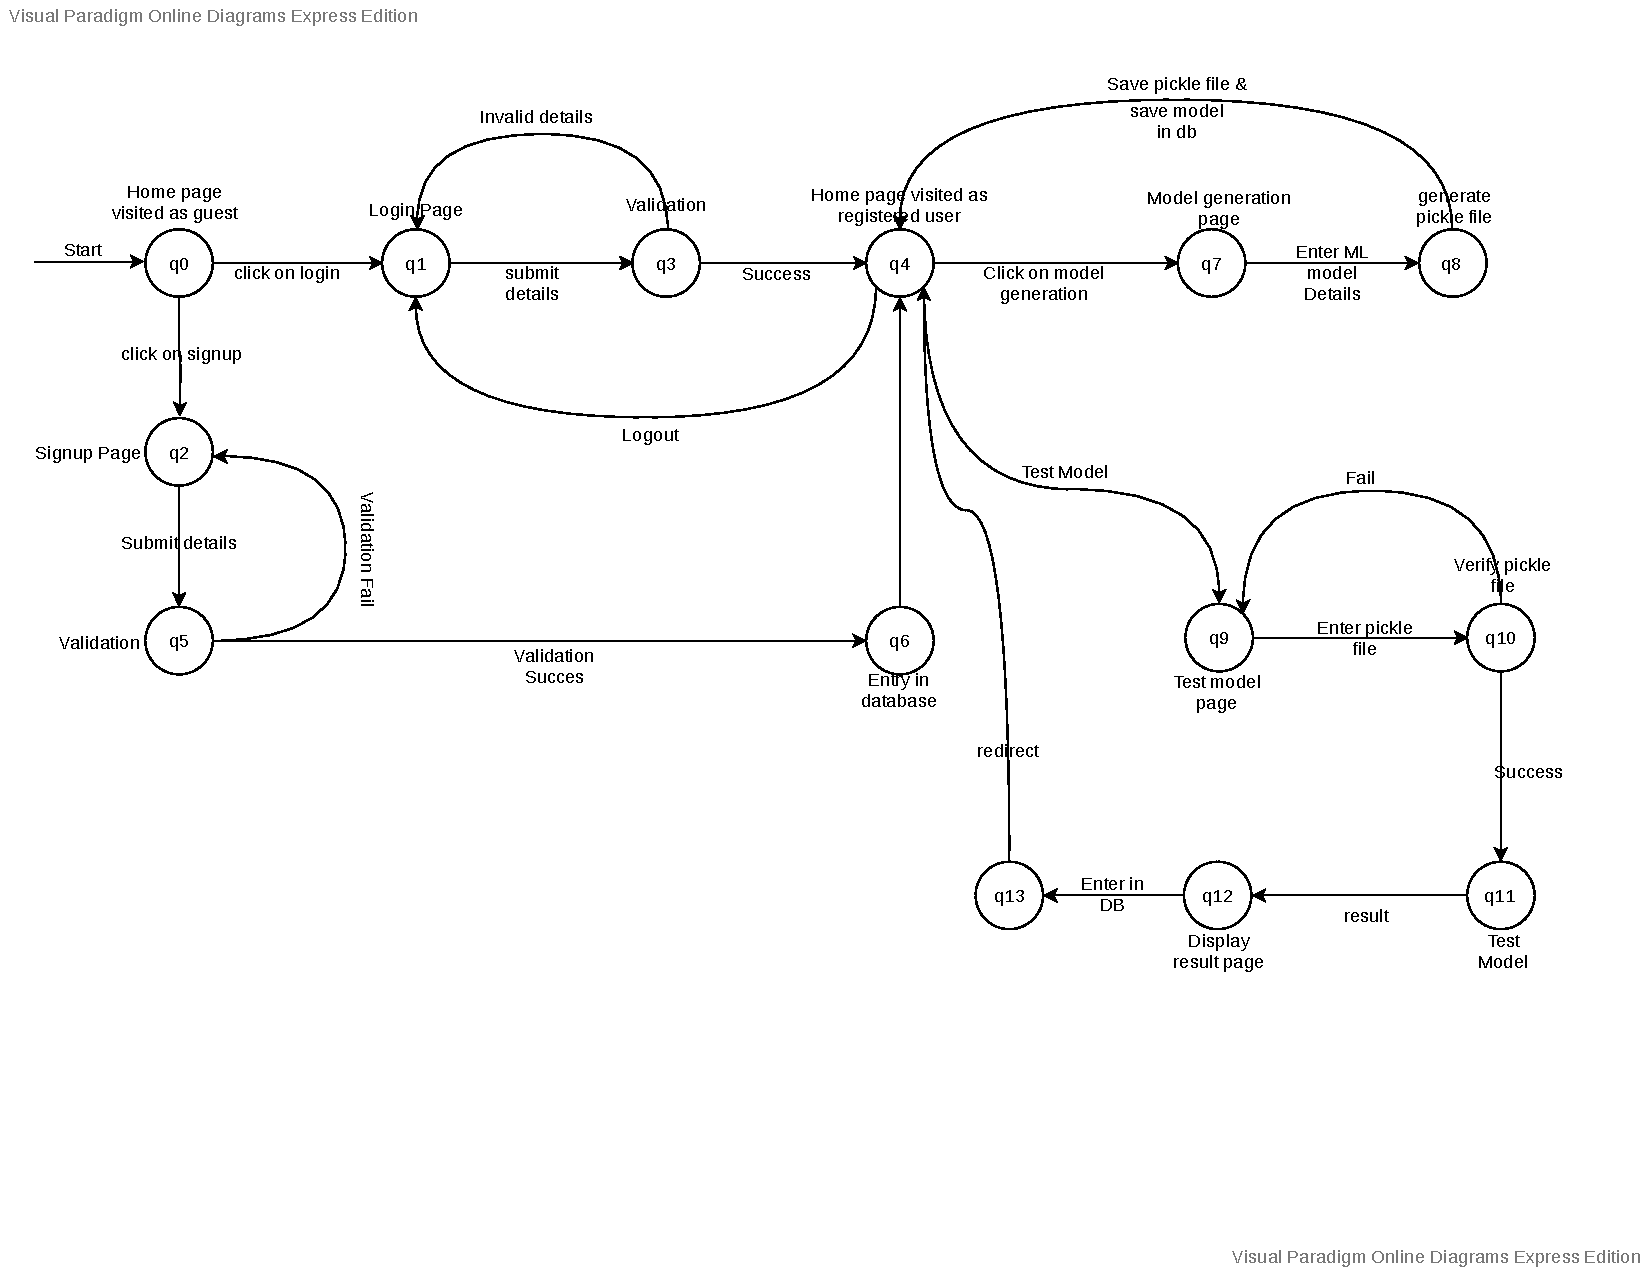
\includepdf[pages=-,pagecommand={}]{../p/FSM.pdf}
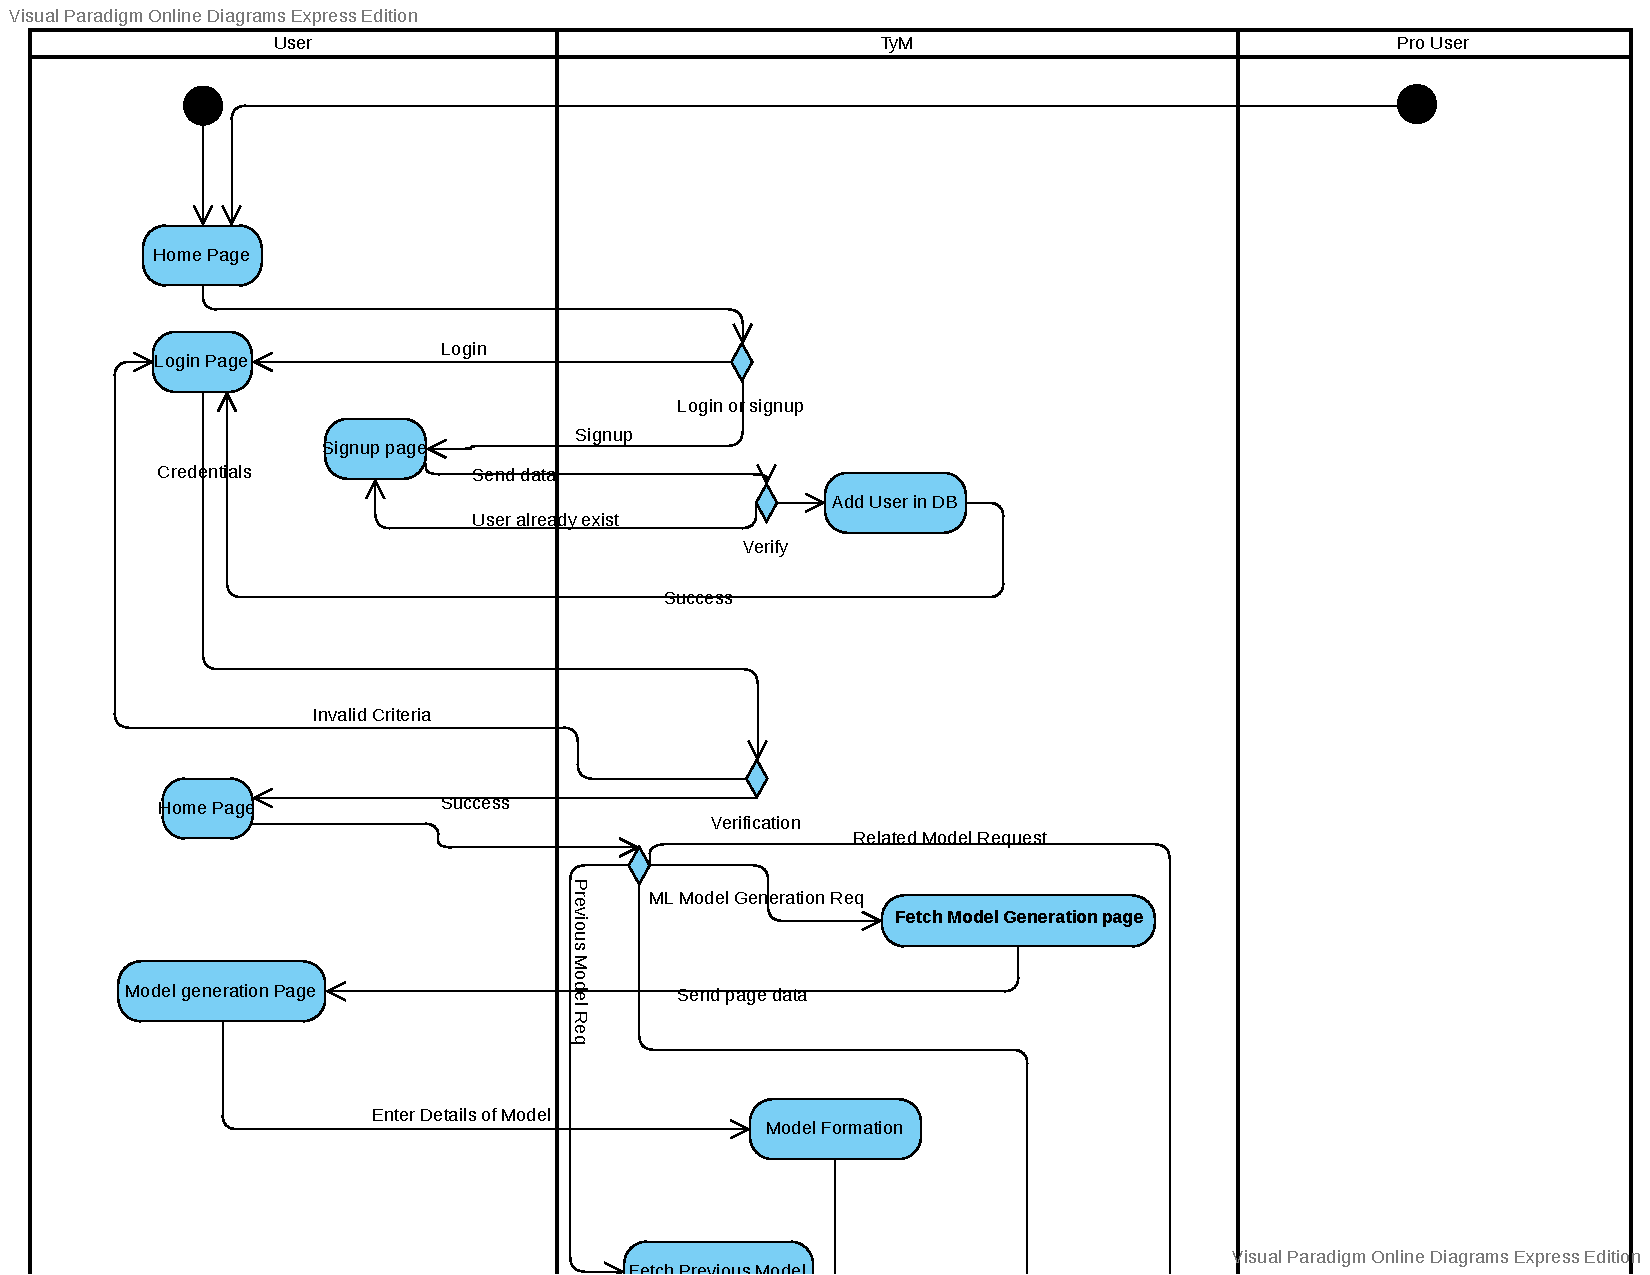
\includepdf[pages=-,pagecommand={}]{../p/ad.pdf}

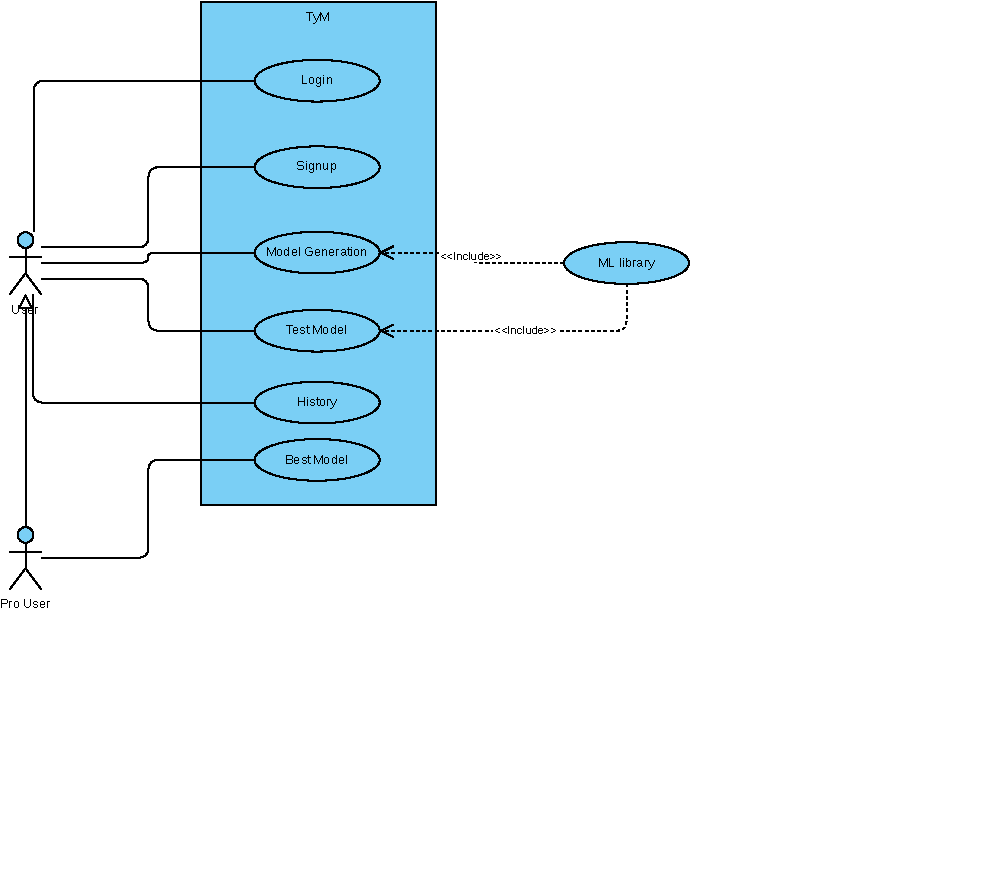
\includepdf[pages=-,pagecommand={}]{../p/uc.pdf}
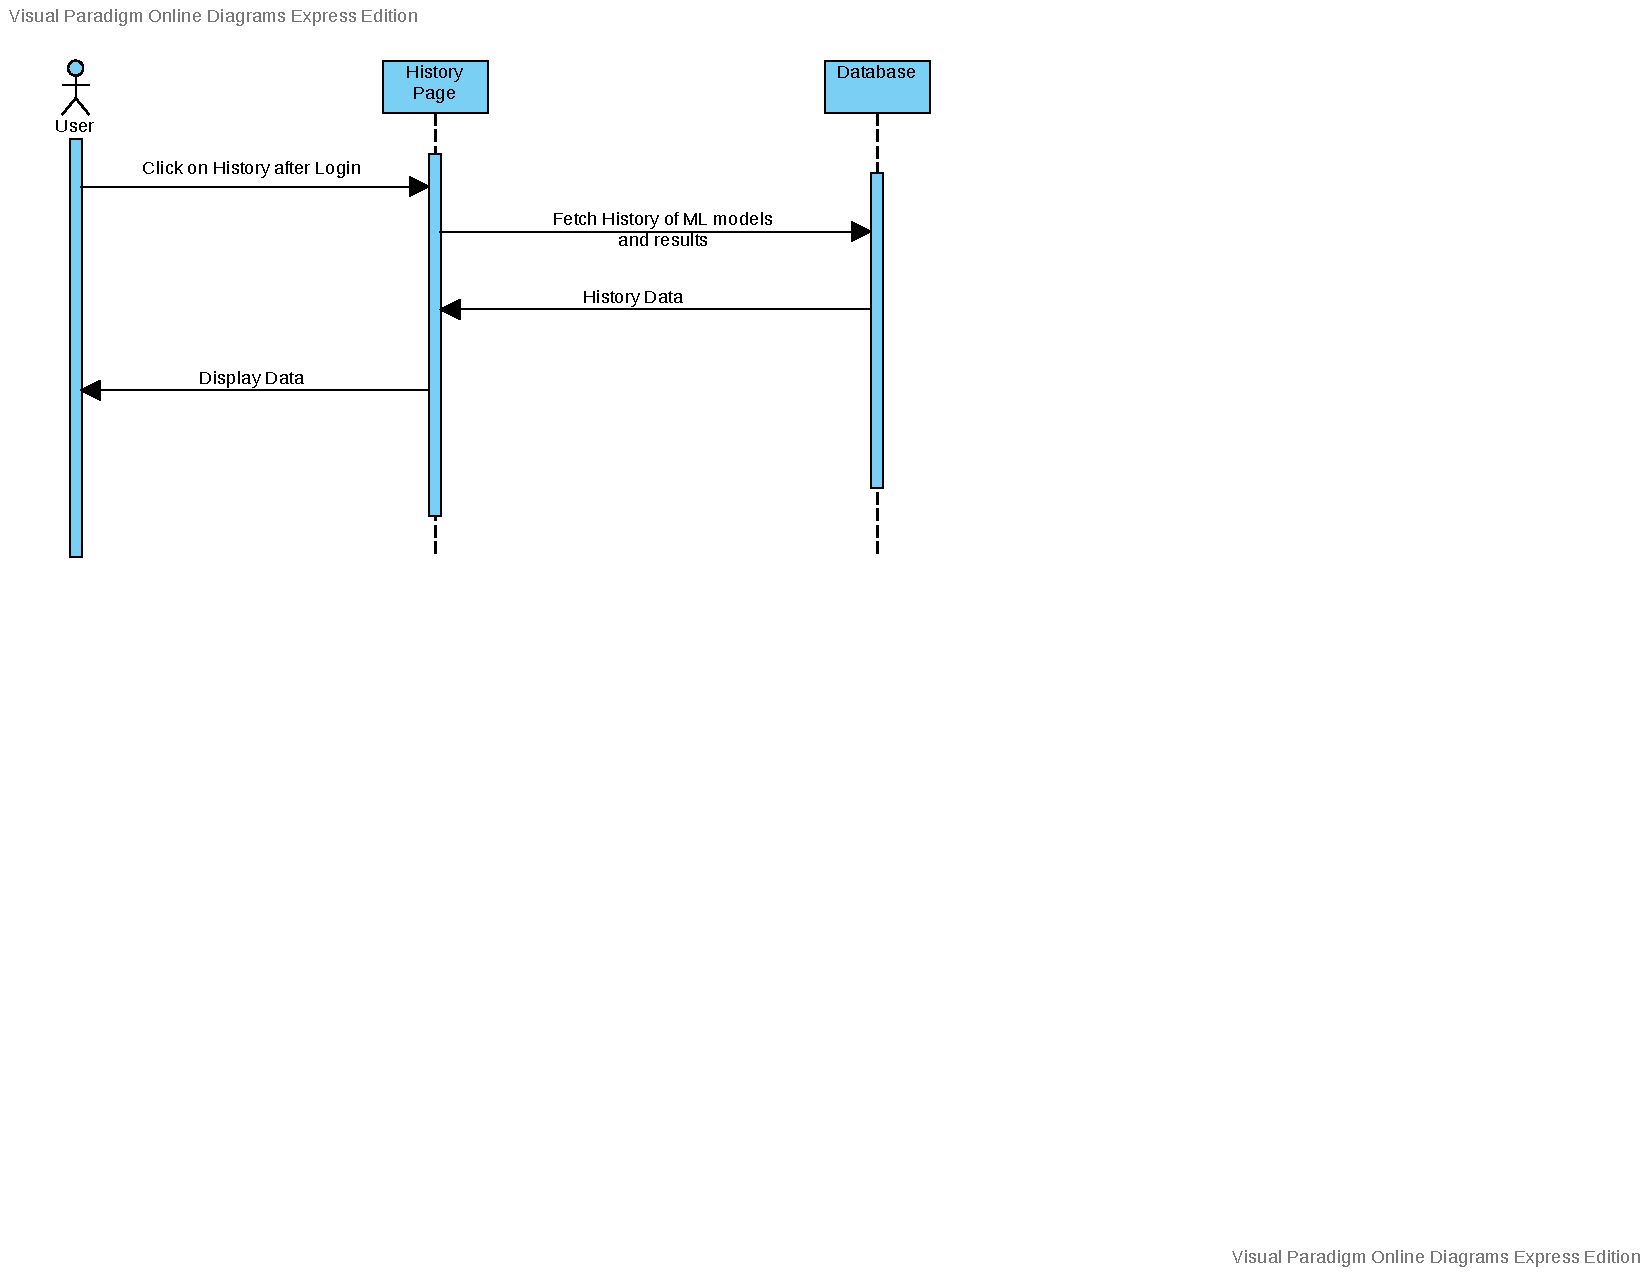
\includepdf[pages=-,pagecommand={}]{../p/s1.pdf}
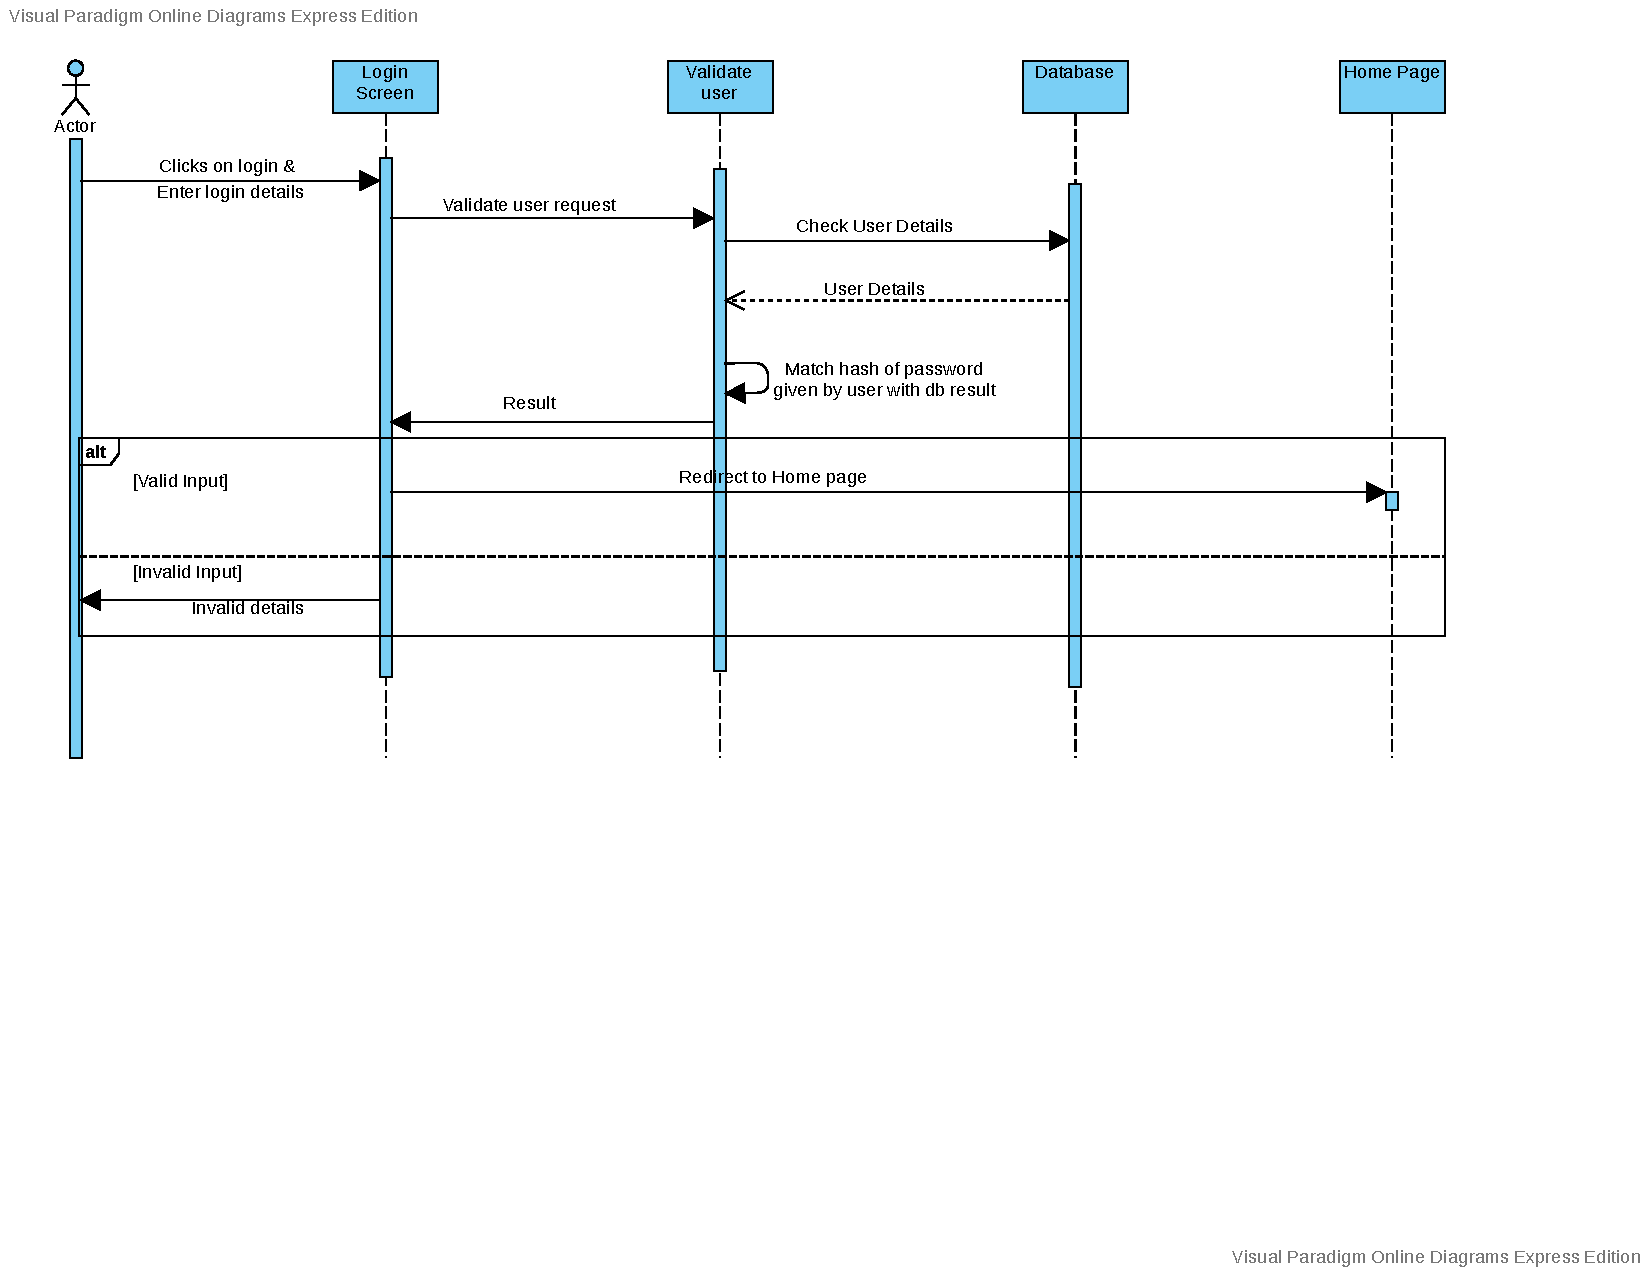
\includepdf[pages=-,pagecommand={}]{../p/s2.pdf}
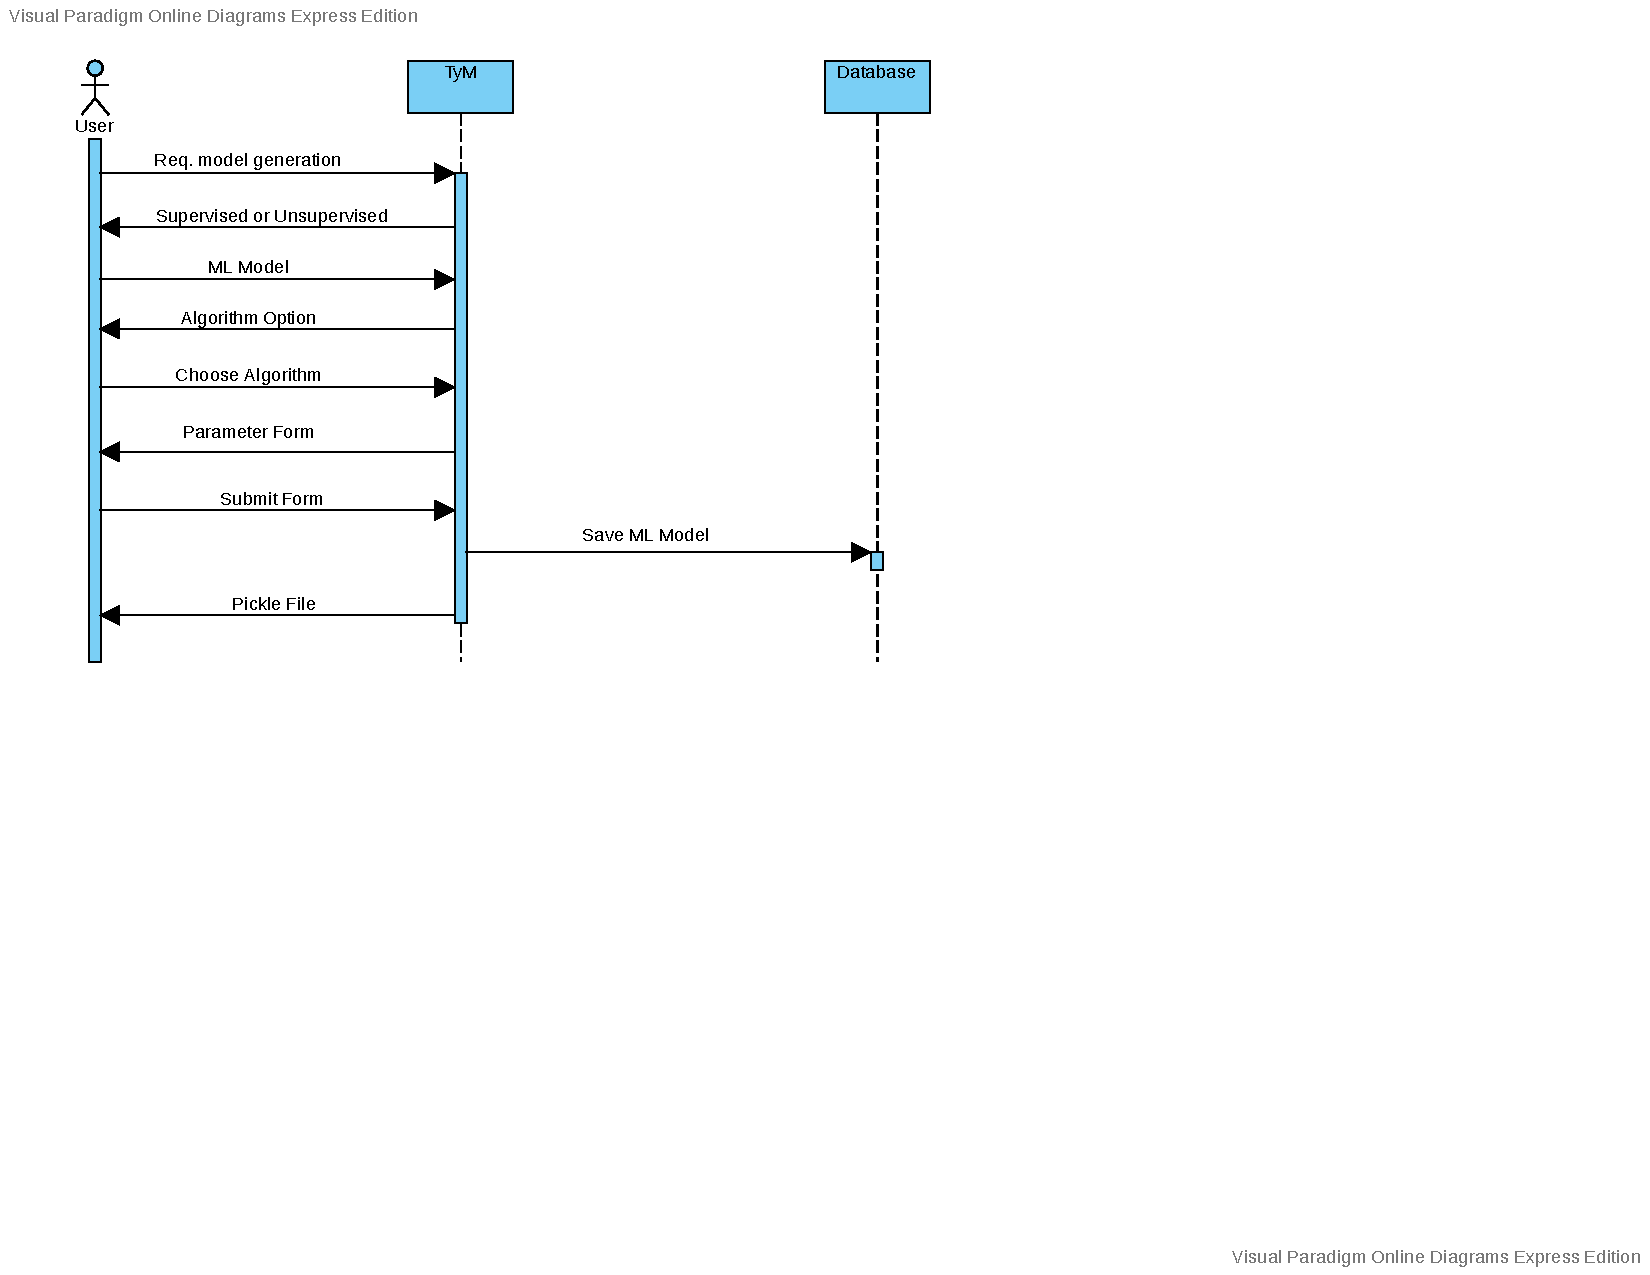
\includepdf[pages=-,pagecommand={}]{../p/s3.pdf}
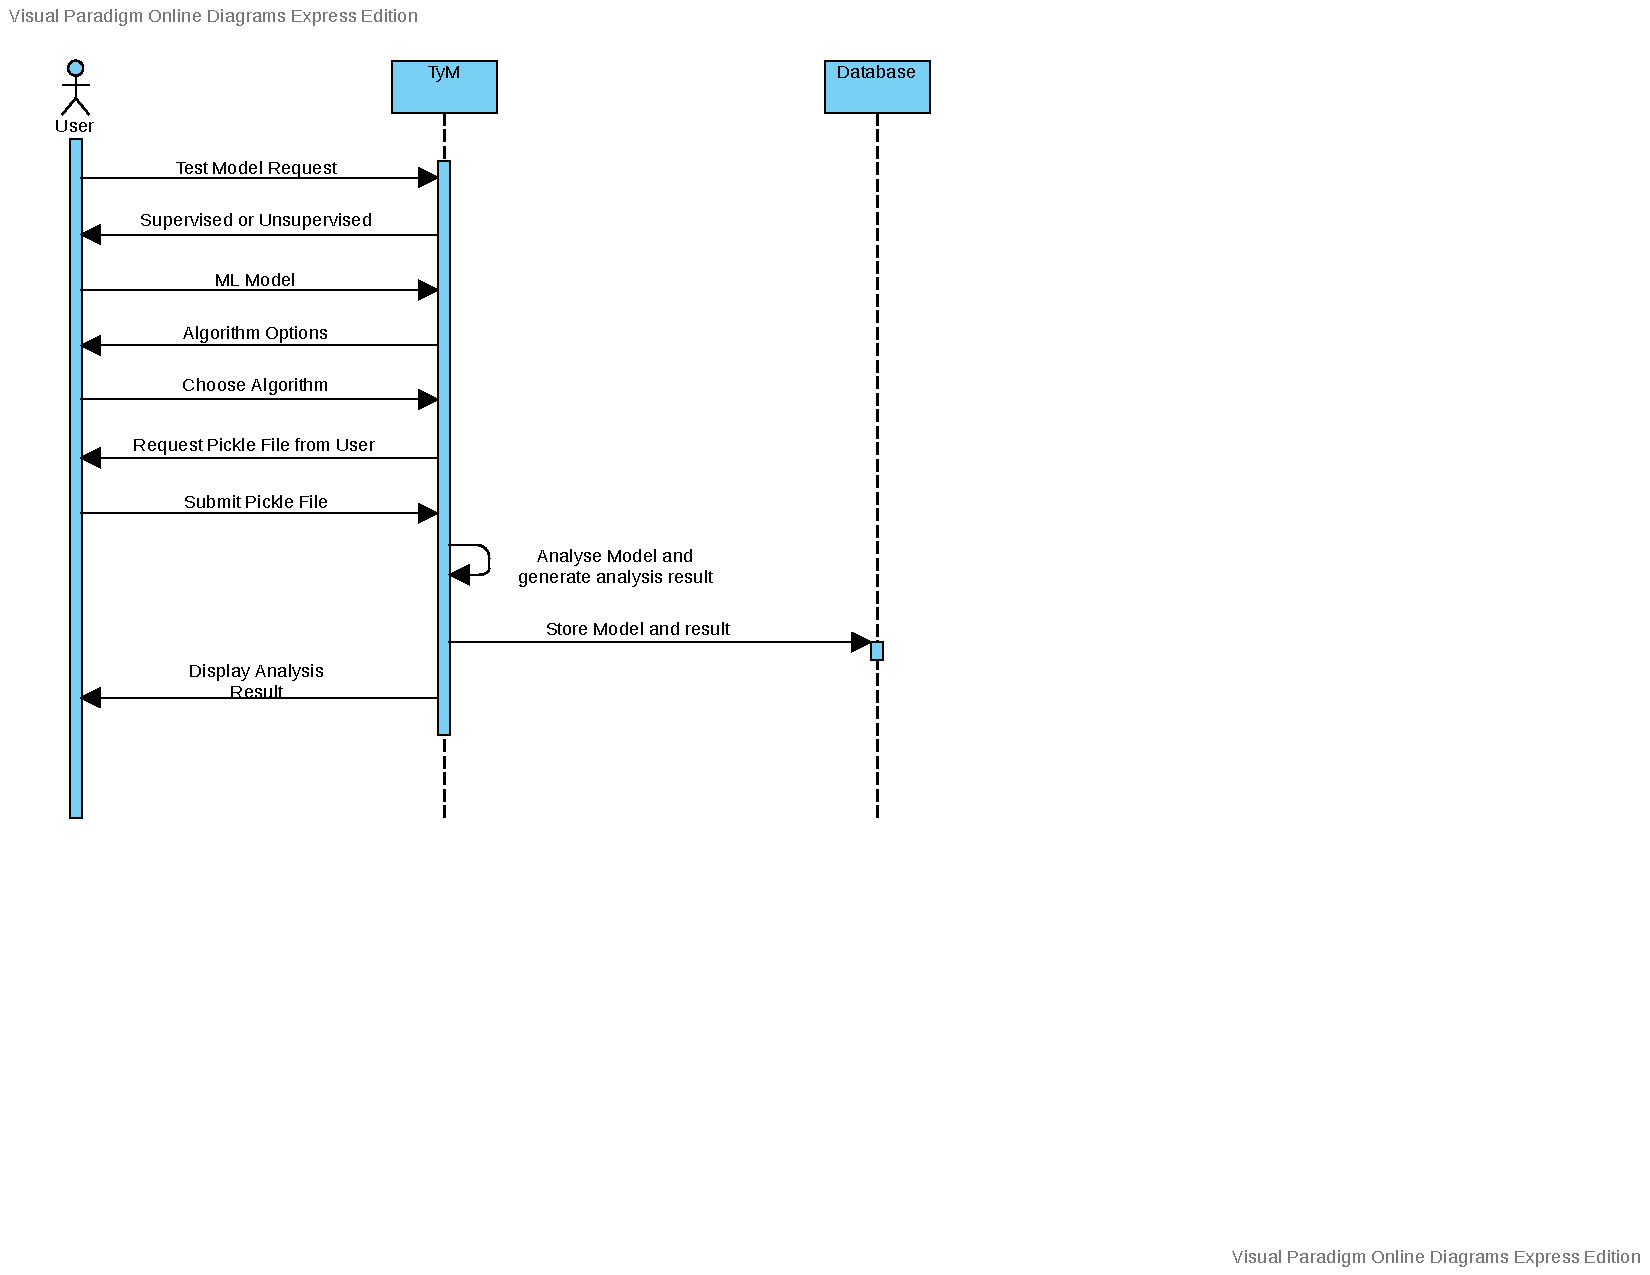
\includepdf[pages=-,pagecommand={}]{../p/s4.pdf}
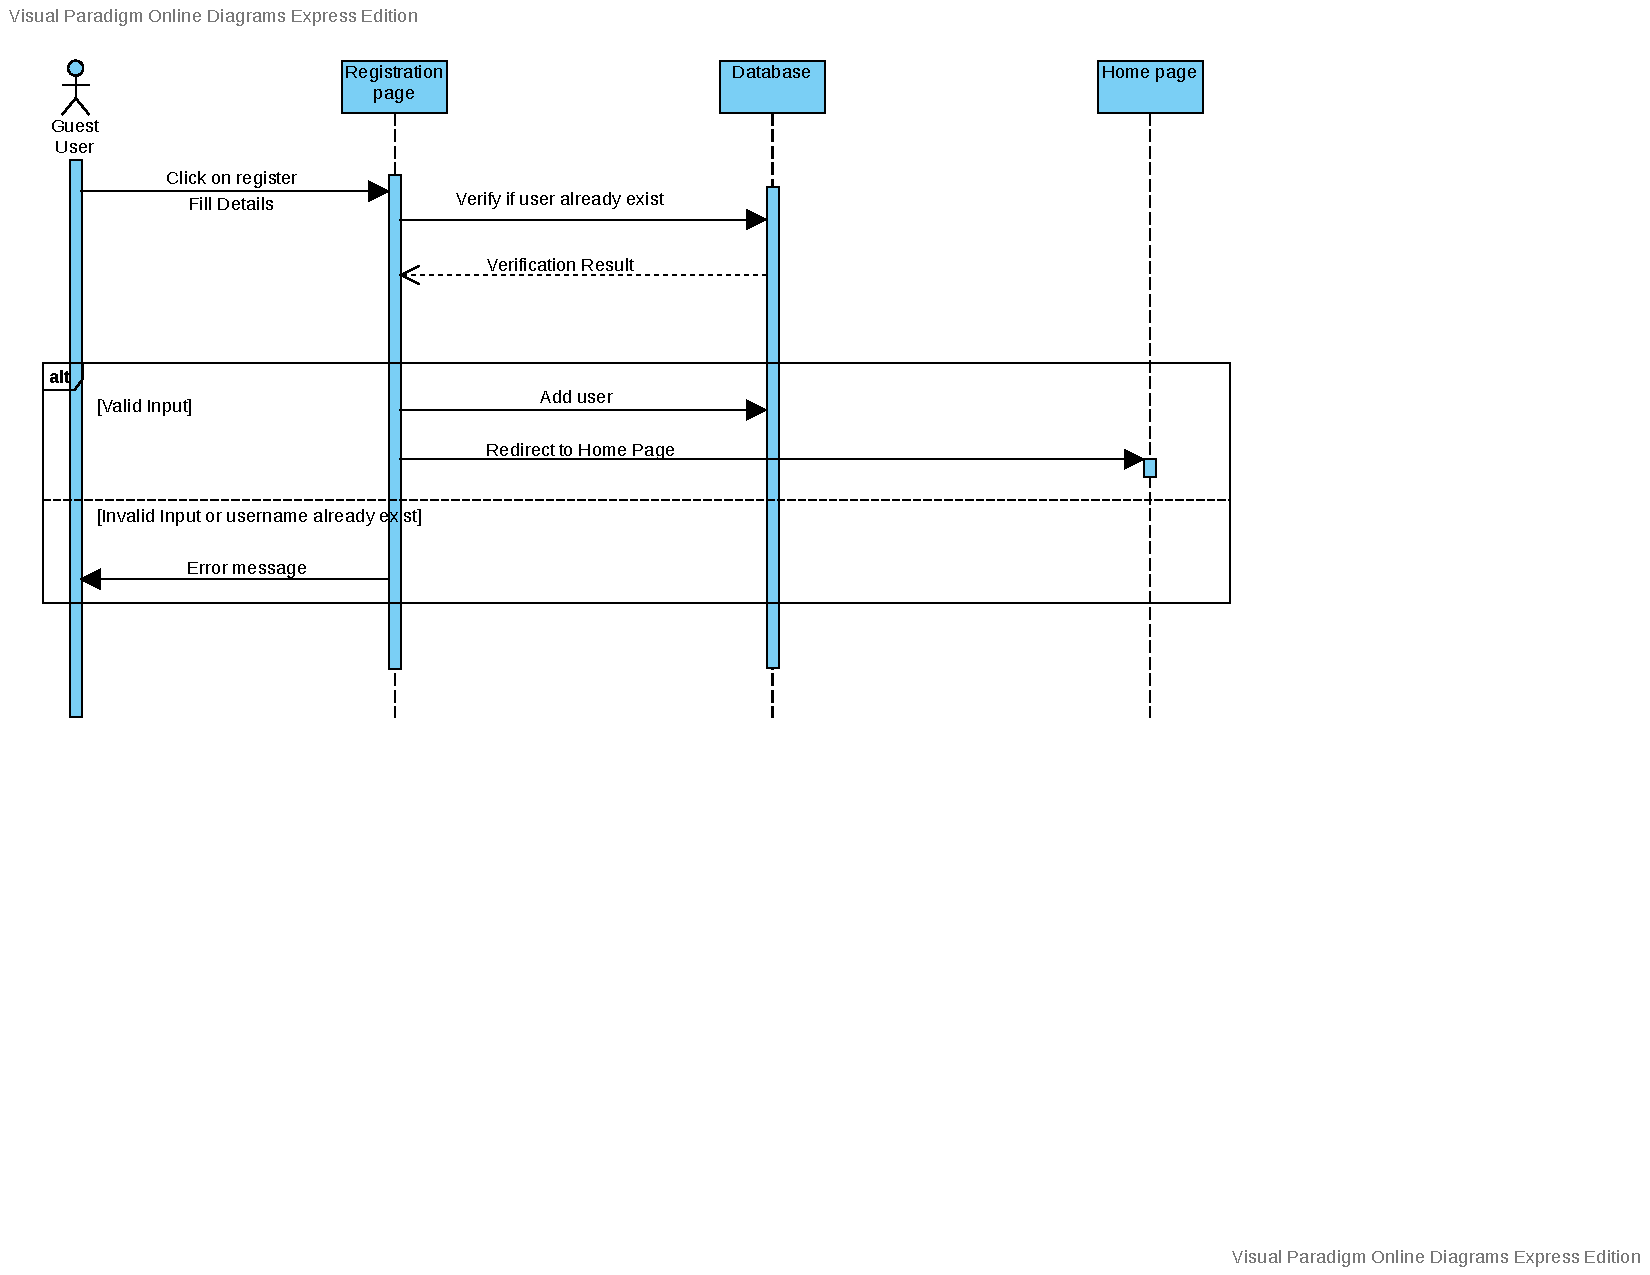
\includepdf[pages=-,pagecommand={}]{../p/s5.pdf}

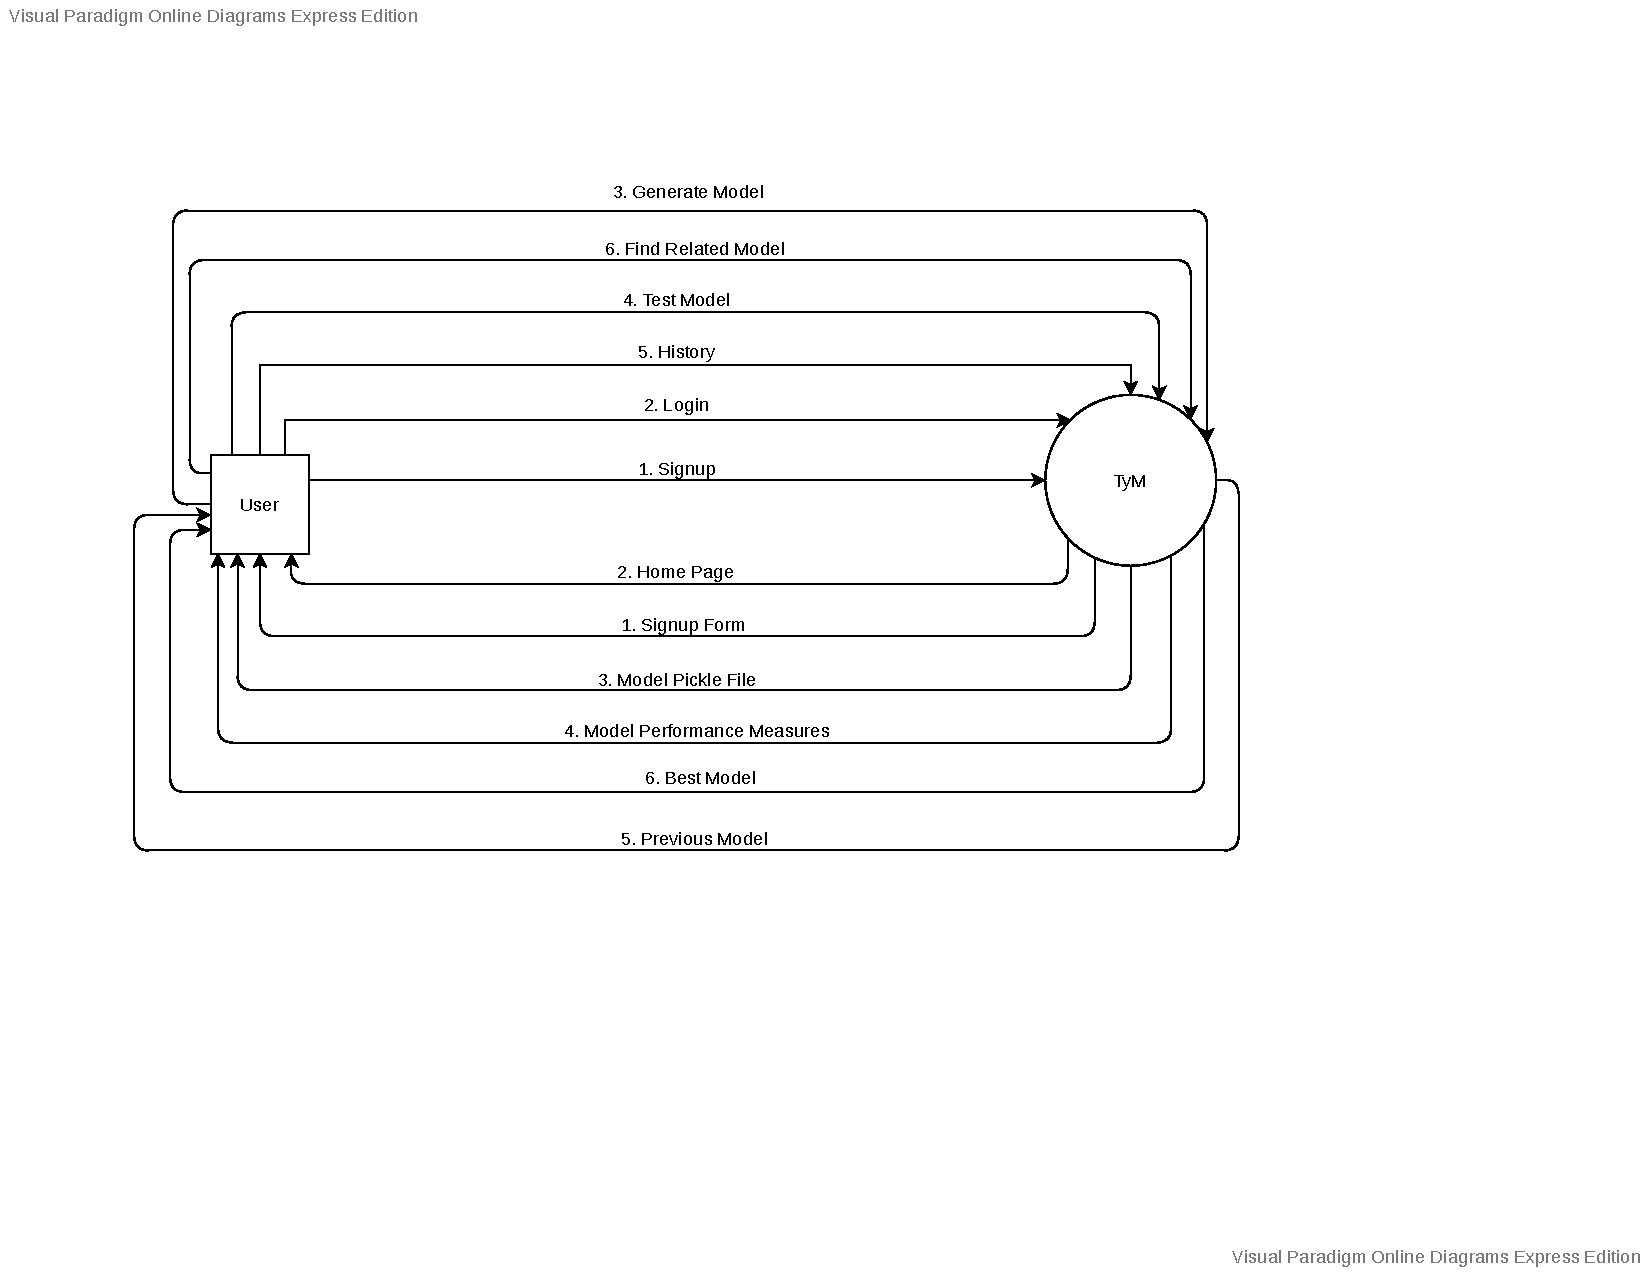
\includepdf[pages=-,pagecommand={}]{../p/context.pdf}
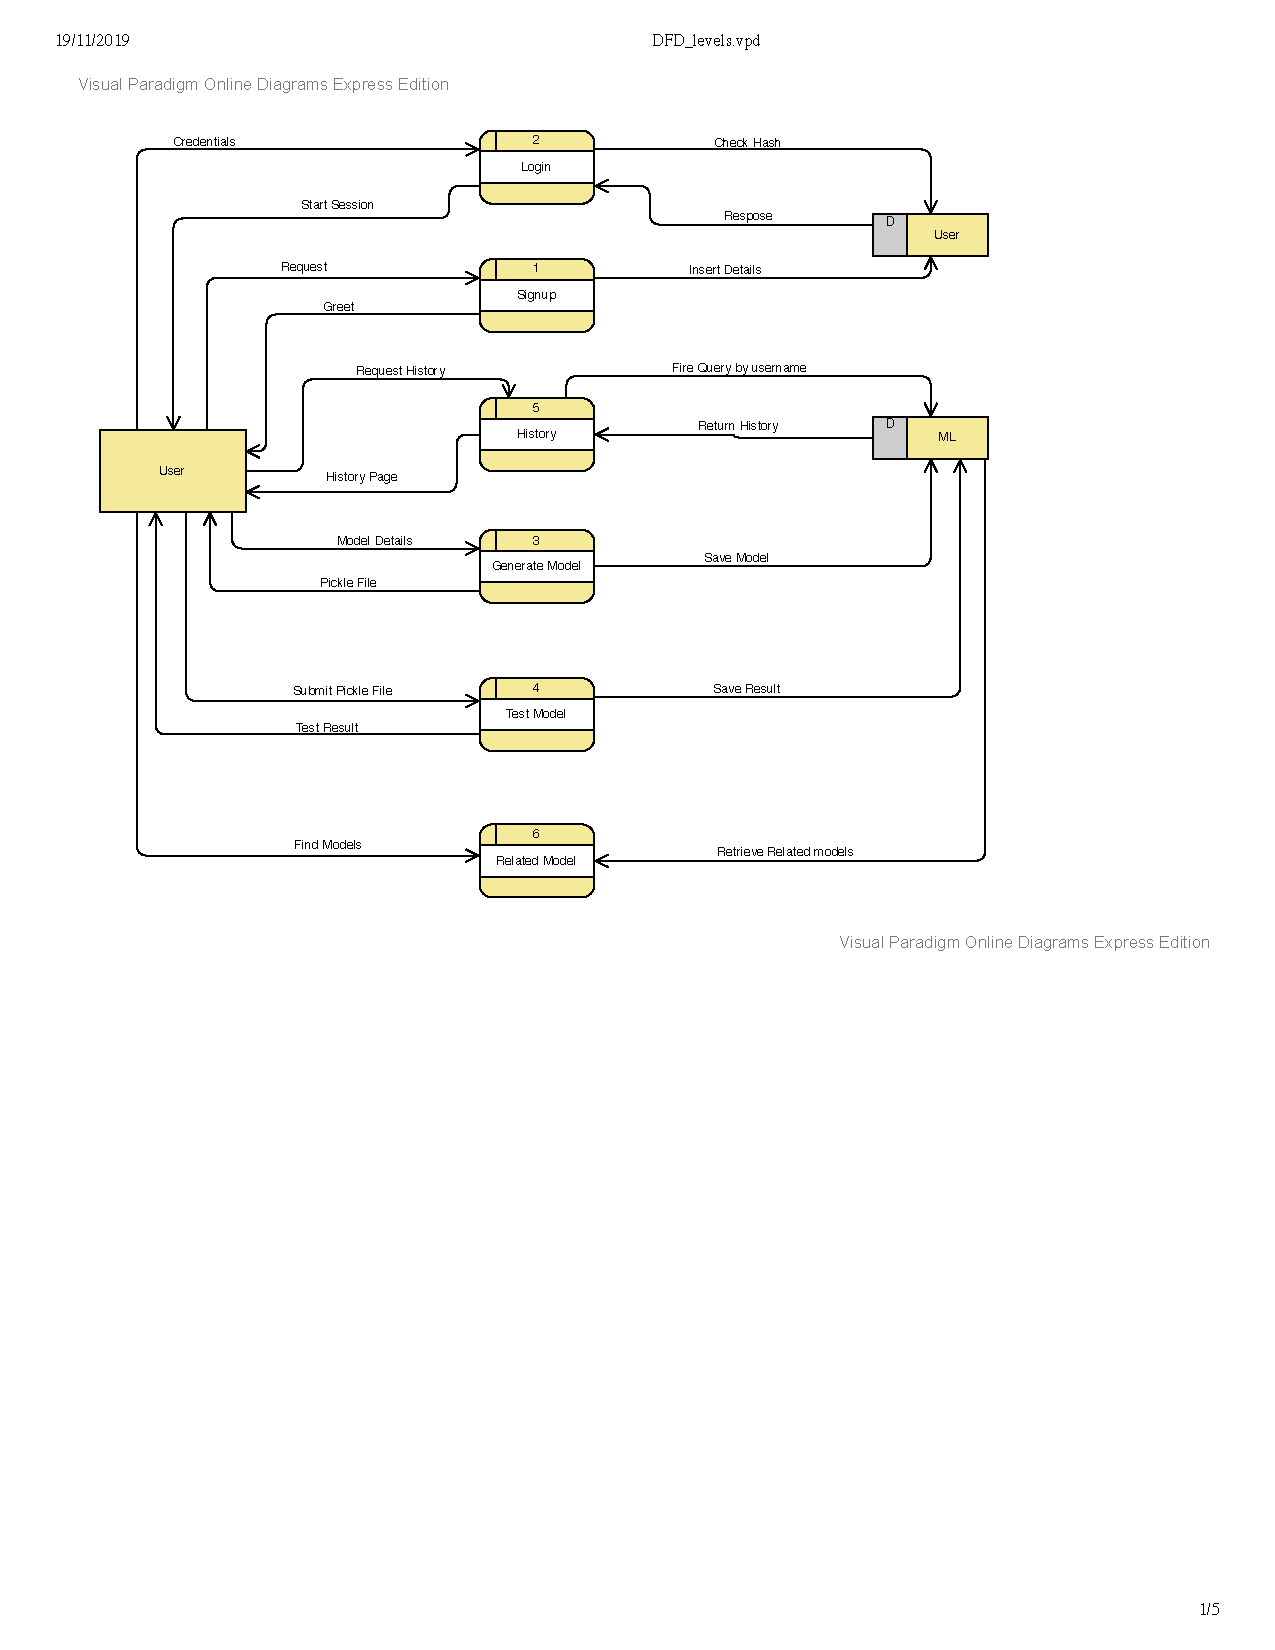
\includepdf[pages=-,pagecommand={}]{../p/dfd.pdf}

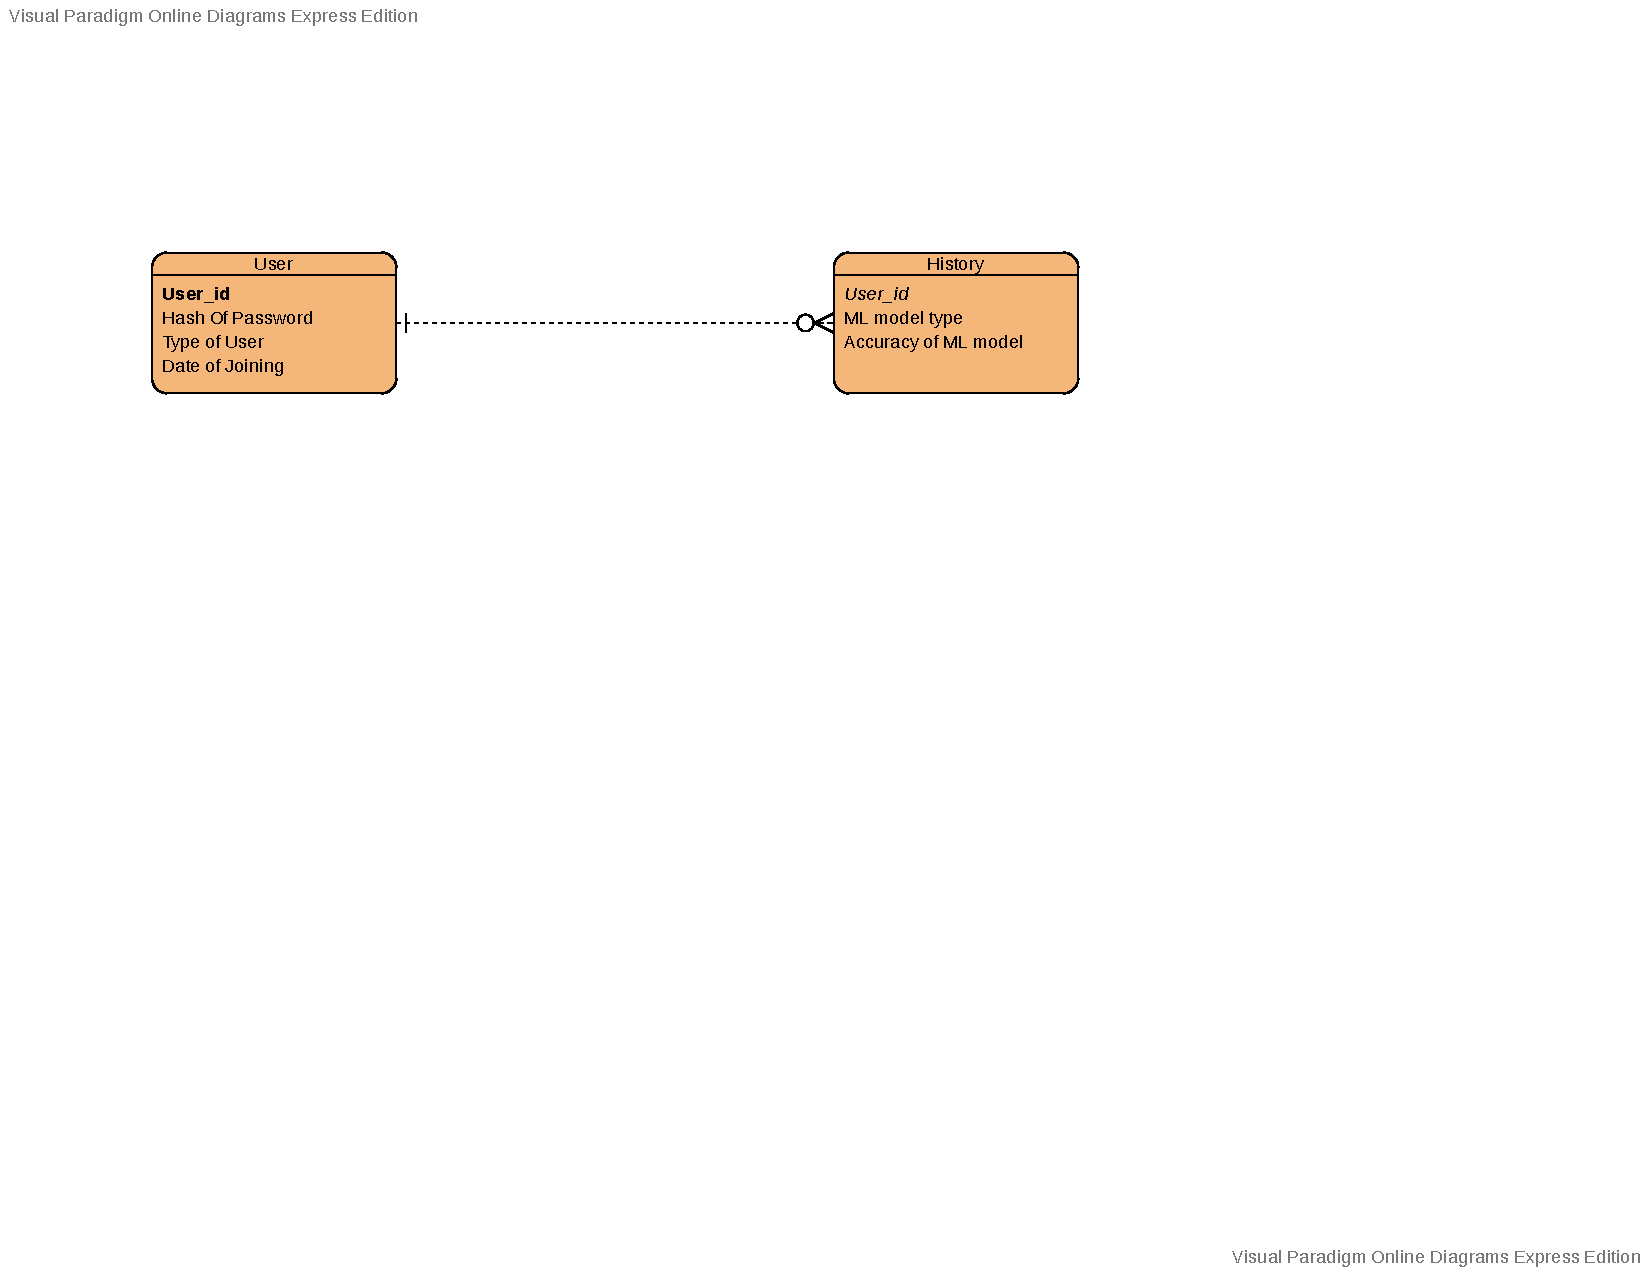
\includepdf[pages=-,pagecommand={}]{../p/er.pdf}

\end{document}
